\section{\pwThree Gameplay Additions}

This section describes the changes and additions \emph{Agile} mode brings to \pwThree.
These additions break the game into four phases requirements, planning, implementation,
and testing. Each phase is designed to introduce some of the concepts of the \emph{Agile} 
process and the software development lifecycle. Players still compete for points, but
the game is broken into three 10 turn rounds called sprints. The game automatically ends
when all three sprints have been completed. Players still build programs to get points,
but the standard mode objectives are replaced by individual requirements with
one objective for each sprint. Completing these objectives awards additional points to
a player that are used in addition to their instruction score to determine a winner.
Each player now chooses their own set of requirements complete and builds their own
customizable deck to help them complete those requirements. Each of the additional
elements and any UI additions or changes will be described in the appropriate
phase below.

\subsection{Game Setup}
In \pwThree the mode dropdown will have an additional entry in it for \emph{Agile} mode.
When selected it will give a short description to let players know their goals will
change to completing individual requirements. When this mode is selected the level
dropdown will be disabled as players will use individual decks with cards related to
the requirement they will choose. However, it may in the future be used to select AI
difficulty levels for the \emph{Agile} mode. As in other modes when an acceptable number
of players has been added the play button will allow players to advance. However,
here players will advance to the requirements phase instead of proceeding straight to
the main game.

\subsection{Requirements Phase}

\begin{figure*}[ht]
	\centering
	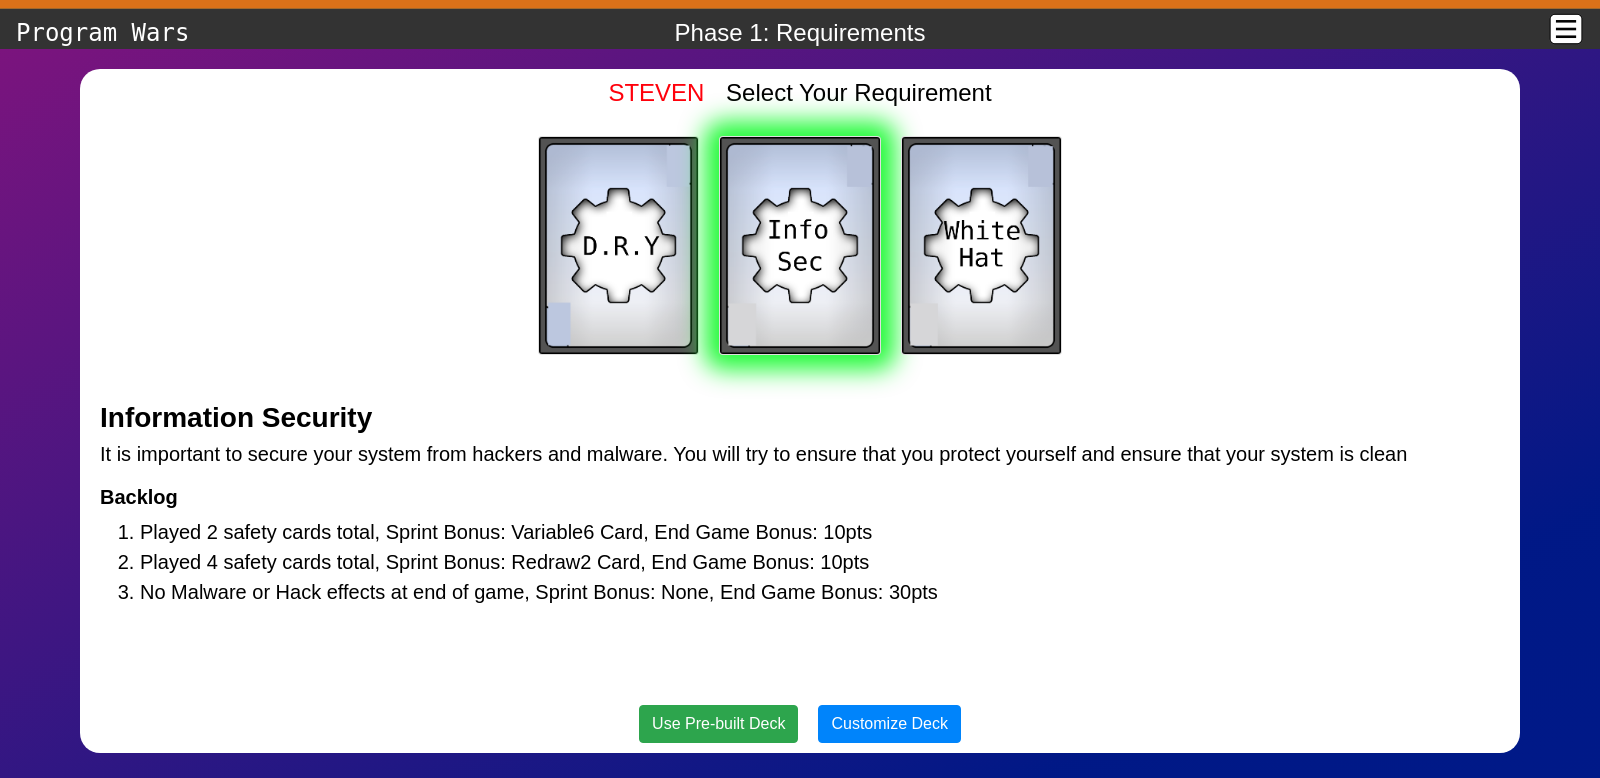
\includegraphics[width=\textwidth]{images/requirement_screen.PNG}
	\caption{The Requirements Phase Screen.}
	\label{fig:requrements}
\end{figure*}

The requirements phase allows players to pick their individual goals for the game.
These requirements are sets of individual objectives that award points and other
bonuses to the player when completed. They represent the requirements that would
be given to a developer or team by a customer for a new software project. Each
requirement has three objectives to complete during the game. Each objective is for
one of the sprints. Completing an objective by the end of the game will award the
player bonus points that will be added to their instruction score and used to determine
the winner. If a player completes an objective before the end of the sprint it is
associated with they will recieve an additional bonus. These bonuses will not be points,
but instead give the player a useful card or status effect. Some sprint bonuses may be
awarded immediately upon completing the objective and others may be awarded at the end
of the sprint, based on how they will help the player.

When players start the requirements phase they will be taken to a new page that has
the available requirements represented as cards. These cards will be on the top portion
of the screen and can be scrolled through and selected to see what their objectives are.
The bottom portion of the screen will give the conditions and bonuses granted for their
completion. When a requirements card is selected it's details will appear here. These
details will indicate the sprint the objective is related to, the bonus points for
completing the objective, and the bonus given for completing the objective before the
end of the sprint. The current prototype for this can be seen in figure???. In the future
a more diverse set of requirements will be added as well as specific card art for each
requirement.

Once a player is satisfied with the requirements they have selected they can advance to
the planning phase where they will customize a deck to help them complete their
requirements. However, an option will exist for players trying out \emph{Agile} mode,
or a new requirement, for the first time to pick a pre-built deck. If all human
players pick pre-built decks the planning phase will be skipped.

\subsection{Planning Phase}

\begin{figure*}[ht]
	\centering
	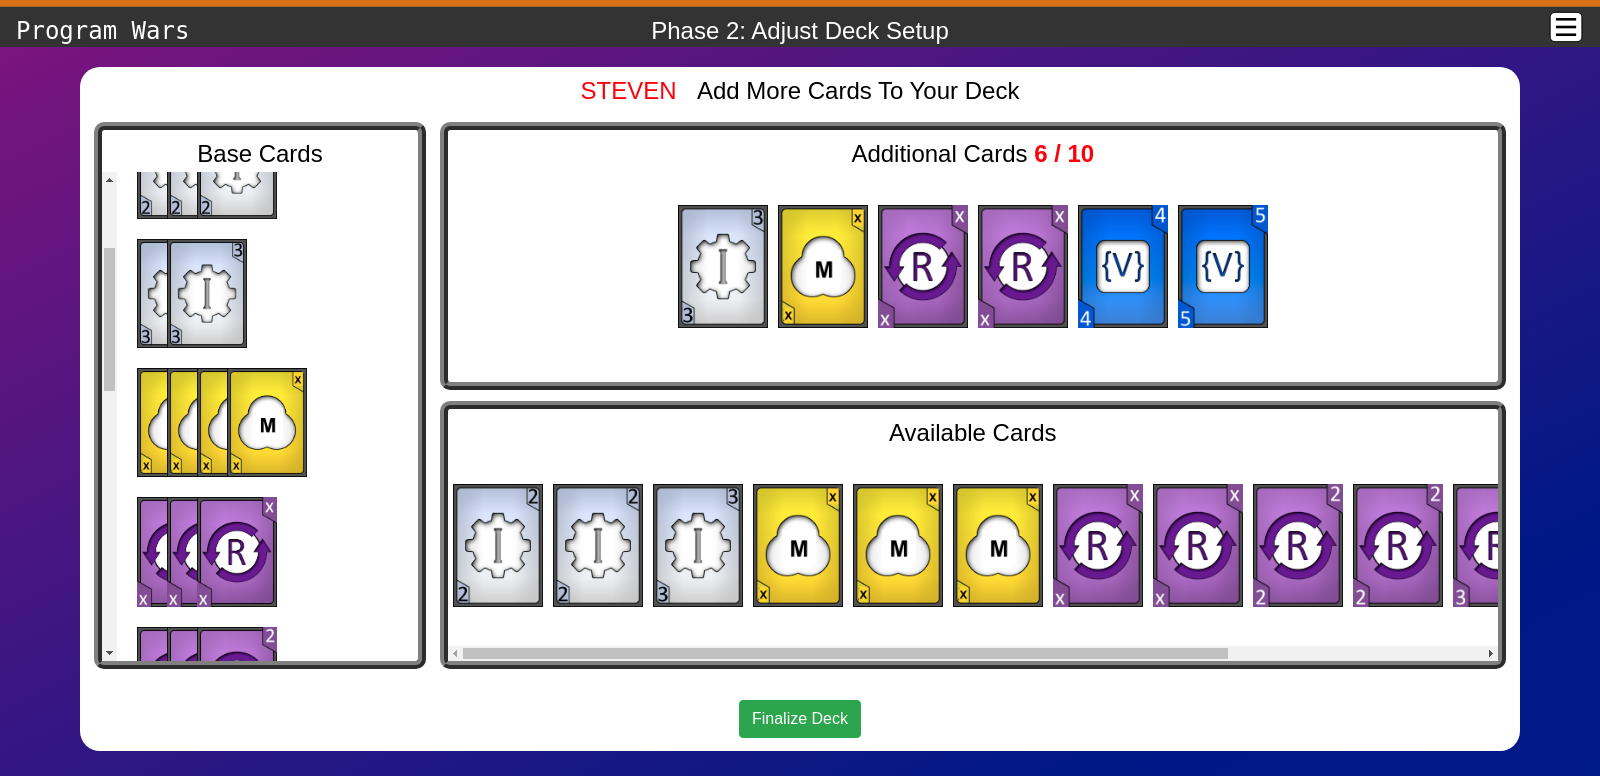
\includegraphics[width=\textwidth]{images/deck_setup_screen.PNG}
	\caption{The Planning Phase Page.}
	\label{fig:deckSetup}
\end{figure*}

Since each of the requirements has different objectives it will be necessary for
players to make some choices about how they can best complete these objectives.
The planning phase represents the part of a software project where developers
make decisions about how the software will be built and what tools they will use.
In the planning phase the player will get a base set of cards for their deck. These
cards are those that are essential for playing \gameNameNS, such as \I and \R cards.
In addition to this they will be given a pool of cards that they can choose a number
of additional cards from. The card pool will be unique to each of the requirements
so that players will have access to certain cards that are most useful for that
requirement. However, it will also have some cards that may not be essential, but
a player may still want as part of their strategy. More powerful cards will be
limited in number and will not appear in the card pools for all requirements.

When players start the planning phase they will be taken to a new page where they
can build their deck. On a portion of left side of the screen there will be a vertical
list of card types. Each type will have a pile showing how many cards of that type,
and value if applicable, will be included in the deck automatically. This way the
player knows what cards are already in their deck and can act accordingly. The rest of
the screen will be split into two horizontal lists of cards. On the top will be the
list of cards to add to the deck, and on the bottom the pool of cards the player can
pick from. Cards can be dragged between these two lists to move them around. The
upper list will have an indicator of how many cards have been added and how many
can be added total. Once a player has added the maximum number of cards to this list
they will be able to advance to the Implementation phase. If there are more than one
human players they will each be given a turn to build their deck.

\subsection{Implementation Phase}
The implementation phase is the name for the actual game in \emph{Agile} mode. For
the most part it play will be the same as it is in standard mode. The major change
is that the game no longer ends when a player reaches a specific point total. Instead
the players each get an equal number of turns through three 10 turn sprints. Once
these sprints are over the game will end. The other major change to the game play
is that completing your requirements is now a key part of winning the game. In standard
mode it is possible to ignore the bonus objectives and win the game. Generally, the
player that reaches the point total first will win. In \emph{Agile} mode the players
will need to complete at least some of their requirements in order to win the game. The
sprint bonuses will also be useful in making it easier to get more points or to
complete subsequent objectives before the end of the game. However, there may be
a set of requirements that focuses on the core aspects of the game and is less
reliant on the bonuses. This will allow beginner players an opportunity to get
used to the format without needing to excell at it immediately.

There will be some small adjustments to the game page's UI for this mode. The
first is that the score limit indicator at the top of the page will be replaced
with one that shows the current sprint and how many turns are left in it. When
a sprint is over an idicator will be given and all end of sprint bonuses that are
due will be given. All other bonuses will be given when they are completed or at
the end of the game.

Second the player information panel will no longer need a score meter. Since there
is no points total to progress toward the score meter and the current score display
will not be useful. They will be replaced with a simple indicator showing the
players instructions score. It will also be useful to have some kind of compact
indicator for the players progress toward the current sprint's objective. For example,
if the player's objective is to build two card stacks that both have nested
loops\footnote{A card stack with two \R cards on it.} the indicator could say
``Nested Loops: 0/2" and update as they built these stacks. This would reduce
the context switching the player would need to do during the game to keep track of
their requirements.

Lastly, in order to allow the player to see a more detailed view of their set of
requirements, a new tab will be added. This replace the standard mode bonus tab.
This tab will show a player each of the sprint objectives they need to complete
as well as any rewards they will receive for completeing them. Like the current
bonus tab awarded bonuses can change color to indicate that they have been given
to the player. There can also be clear indicators of progress for each objective.

When all three sprints have ended the game will advance to the testing phase.

\subsection{Testing Phase}
The testing phase is a replacement for the winner's modal that is displayed at
the end of beginner and standard modes. This phase represents a kind of acceptance
testing phase for the program the player built. The player had requirements to
fulfill for the project so they are judged on their progress. This is where the
bonus points for requirements will be added to a player's instruction score. The
detailed progress for each player toward their requirements will be shown. Here
human players will be able to see how close an AI player came to completing their
requirements. The player with the most points will be the winner. Tie breaks will
favour the player that completed more requirements in total or by the end of the
appropriate sprint. The points given for requirements should be balanced to allow
strategies that do not focus as much on instruction score to be competetive if
they are completed.


